\chapter{Astrophysical Radiation}
\label{chapter:astro_rad}

As discussed in Chapter~\ref{chapter:eor_intro}, the target signal of EoR experiments has a brightness temperature of order $\sim 10$\,mK. At the $50--200$\,MHz frequencies for these experiments, however, foreground radiation from the Milky Way (referred to as `the Galaxy', with a capital `G' for much of this thesis), extragalactic sources and manmade interference  is the principle challenge to overcome. In this Chapter, I outline our current understanding of polarized and unpolarized foregrounds, and the implications for the dynamic range required for an EoR detection. For a comprehensive review of radiative processes in astrophysics, see \cite{Rybicki.79}.

\section{Synchrotron Radiation}

Any accelerating charged particle will radiate. For low-frequency radio foregrounds, the radiation we are most interested in is emitted by electrons accelerated by Galactic magnetic fields.
At non-relativistic velocities, the radiation of a charged particle accelerated by magnetic field $\vec{B}$ is well-described by relatively simple formulae, and is referred to as `cyclotron radiation'. In this case, the emission spectrum is simply determined by gyration frequency about the magnetic field lines.
At relativistic velocities, the spectrum becomes more complicated, and is referred to as `synchrotron radiation'.

The equation of motion of a relativistic charged particle of mass $m$, charge $q$ and velocity $\vec{v}$ can be written as 
\begin{equation}
\frac{{\rm d}}{{\rm d}t}(\gamma m \vec{v}) = \frac{q}{c}\vec{v}\times\vec{B},
\label{eq:astropol_eom_b}
\end{equation}
where $\gamma$ is the Lorentz factor, and
\begin{equation}
\frac{{\rm d}}{{\rm d}t}(\gamma m c^2) =q \vec{v}\cdot\vec{E} = 0,
\label{eq:astropol_eom_e}
\end{equation}
where $\vec{E}$ is the electric field. Equation~\ref{eq:astropol_eom_e} implies that either $\gamma$ or $|\vec{v}|=v$ are constant. Therefore, we may write
\begin{equation}
\gamma m\frac{{\rm d}\vec{v}}{{\rm d}t} = \frac{q}{c}\vec{v}\times\vec{B}.
\end{equation}
Decomposing the velocity into components perpendicular and parallel to $\vec{B}$,
\begin{equation}
\frac{{\rm d}\vec{v}_{\parallel}}{{\rm d}t} = 0;\,\,\,\,\,\frac{{\rm d}\vec{v}_{\perp}}{{\rm d}t} = \frac{q}{\gamma m c} \vec{v}_{\perp}\times\vec{B},
\end{equation}
we find that $\vec{v}_{\parallel}$ is constant, and as $v$ is constant, so $\vec{v}_{\perp}$ must be also. This proves that motion along the magnetic field lines is helical, with gyration frequency
\begin{equation}
\omega_B = \frac{qB}{\gamma m c}.
\end{equation}
Using the covariant form of the Larmor Formula with the magnitude of acceleration perpendicular to the magnetic field $a_{\perp} = \omega_B v_{\perp}$, the total emitted radiation has power
\begin{equation}
P = \frac{2 q^2}{3c^3}\gamma^4 a_{\perp}^2,
\end{equation}
which when accounting for an isotropic velocity distribution, reduces to
\begin{equation}
P = \frac{4}{24\pi}\sigma_T c \beta^2 \gamma^2 B^2
\end{equation}

Since the electrons follow a helical path, an observer will only see components of the emission when the motion is parallel to the line-of-sight. The observed radiation will be emitted along path $\delta s$ with radius of curvature $r$ and and angle $\delta \theta$, such that $\delta\theta = 2/\gamma$ and $\delta s = 2r/\gamma$. Equations~\ref{eq:astropol_eom_b} and \ref{eq:astropol_eom_e} grant
\begin{equation}
r = \frac{v}{\gamma\omega_B\sin\alpha},
\end{equation}
where $\alpha$ is the angle between $\vec{v}$ and $\vec{B}$. The time taken for the electron to travel $\delta s$, and therefore emit the observed radiation, may be characterized by a critical frequency
\begin{equation}
\omega_c = \frac{3}{2}\gamma^3\omega_B\sin\alpha.
\end{equation}

Deferring to \cite{Rybicki.79} for a full discussion, the frequency spectrum of synchrotron radiation is intimately tied to the helical geometry of the problem and $\omega_c$, with power per unit frequency proportional to some function $F(\omega/\omega_c)$:
\begin{equation}
P(\nu) = \frac{\sqrt{3}q^3B\sin\alpha}{m_e c^2}F(\frac{\omega}{\omega_c})
\label{eq:astropol_sync_power}
\end{equation}
where the form of $F$ depends on the energy distribution of the electrons. For black-body radiators in the Rayleigh-Jeans limit, appropriate for low-frequency radio observations, the number density of particles with energy $E$ can be described with a power law:
\begin{equation}
N(E){\rm d}E = AE^{-p}{\rm d}\gamma ,
\end{equation}
where $A$ is a constant of proportionality that can vary with angle of observation. In this case, it can be shown that the total energy density per unit frequency is
\begin{equation}
P(\nu) = \frac{A\sqrt{3}q^3B\sin\alpha}{m_e c^2 (p+1)}\left(\frac{2\pi mc}{3qB\sin\alpha}\nu\right)^{-{\frac{p-1}{2}}}\Gamma\left(\frac{p}{4} + \frac{19}{12}\right)\Gamma\left(\frac{p}{4} - \frac{1}{12}\right).
\end{equation}

The objective of this exercise was to show that the total power of synchrotron radiation is innately smooth as a function of frequency; it can be described as a power law. An example observation of low-frequency Galactic synchrotron is shown in Figure~\ref{fig:astropol_edges_spec}. The observed sky spectrum has a spectral index $\beta_*=2.52\pm0.04$ for brightness temperature $T(\nu)\propto\nu^{-\beta_*}$. Recall that the {\sc hi} EoR field has a complex structure in both the image plane and along the line-of-sight (c.f. Figure~\ref{fig:eor_intro_plp_sim}). The superposition of emission lines from this field will lead to unsmooth, structured emission per unit frequency.
In the face of synchrotron foregrounds being many orders of magnitude brighter than the 21\,cm emission, \textit{this difference in spectral behavior is the single most important distinguishing feature between foregrounds and the EoR}.

\begin{figure}
\centering
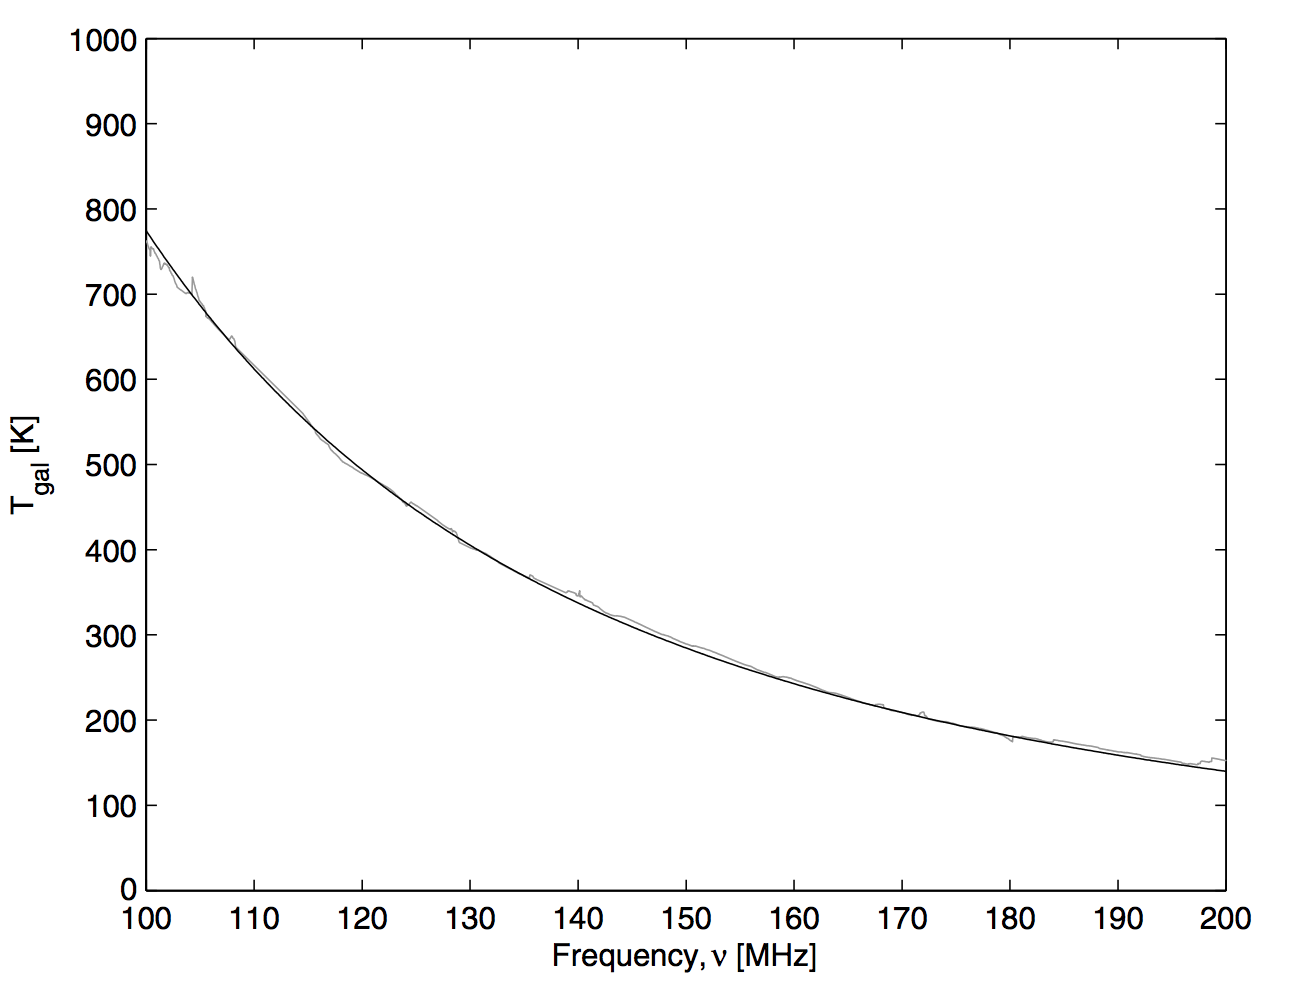
\includegraphics[width=0.75\textwidth]{chapters/astropol/figures/edges_spectrum.png}
\caption[The low-frequency synchrotron spectrum of the sky, as measured by \cite{Rogers.08}.]{The low-frequency synchrotron spectrum of sky, measured by \cite{Rogers.08}. Their measurement is shown in light grey, overlaid with a well-fit power law of spectral index $2.52\pm0.04$.}
\label{fig:astropol_edges_spec}
\end{figure}

\section{Stokes parameters}

It is extremely unlikely that we will observe radiation from electrons spiralling along magnetic field lines that are exactly parallel or perpendicular to our line-of-sight. Instead, some elliptically polarized component of the radiation is observed. The Stokes parameters are quantities used to describe the polarization state of electromagnetic waves.

We can describe a monochromatic electromagnetic wave propagating towards the observer as the real part of 
\begin{equation}
\vec{E} = \vec{E}_0e^{-i\omega t} = \begin{pmatrix}
E_1 e^{i\phi_1}\\
E_2 e^{i\phi_2}
\end{pmatrix}e^{-i\omega t}
\end{equation}
It can be shown \citep[e.g.][]{Rybicki.79} that the real part of the vector above can be mapped, in general, to the principle axes of an ellipse at angles $\psi$ and $\chi$ to the Cartesian grid, as shown in Figure~\ref{fig:astropol_pol_ellipse}. These two angles, $E_1$, and $E_2$, can be used to define the Stokes parameters for monochromatic waves:
\begin{eqnarray}
I \equiv E_1^2 + E_2^2 = E_0^2
Q \equiv E_1^2 - E_2^2 = E_0^2\cos 2\psi \cos 2\chi
U \equiv 2E_1E_2\cos(\phi_1 - \phi_2) = E_0^2\cos 2\chi \sin 2\psi
V \equiv 2E_1E_2\sin(\phi_1 - \phi_2) = E_0^2\sin 2\chi
\end{eqnarray}

\begin{figure}
\centering
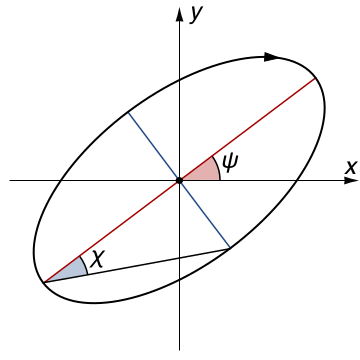
\includegraphics[width=0.5\textwidth]{chapters/astropol/figures/pol_ellipse.png}
\caption{A representation an elliptically polarized monochromatic wave with respect to the Cartesian grid.}
\label{fig:astropol_pol_ellipse}
\end{figure}

% what is polarization (emag) -- STOKES PARAMETER DEFINITIONS

\section{Total intensity foregrounds}

% GSM 2008, 2017
% GLEAM
% compare to 21cm amplitude

%The major challenge that faces all 21 cm experiments
%is isolating a small signal that is buried underneath foregrounds
%and instrumental systematics that are, when
%combined, four to five orders of magnitude brighter (e.g.,
%Santos et al. 2005; Ali et al. 2008; de Oliveira-Costa
%et al. 2008; Jeli´c et al. 2008; Bernardi et al. 2009, 2010;
%Ghosh et al. 2011; Pober et al. 2013; Bernardi et al.
%2013; Dillon et al. 2014; Kohn et al. 2016)

\section{Linearly Polarized Foregrounds}
% sources of astrophysical polarization
% magnetic fields and rotation measures - REMARK UPON UNSMOOTHNESS
% oppermann map -- high RM point sources
% Lenc, Jelic, etc. diffuse low RM stuff -- RELATIVE POWER BETWEEN STOKES PARAMETERS
% sources of depolarization:
%% beam
%% heat(?)
%% ionosphere
% compare again to 21cm, insofar that it SHOULD BE ZERO IN Q U V